
% Thank you Josh Davis for this template!
% https://github.com/jdavis/latex-homework-template/blob/master/homework.tex

\documentclass{article}

\newcommand{\hmwkTitle}{Final Report}

% % ----------

% Packages

\usepackage{fancyhdr}
\usepackage{extramarks}
\usepackage{amsmath}
\usepackage{amssymb}
\usepackage{amsthm}
\usepackage{amsfonts}
\usepackage{tikz}
\usepackage[plain]{algorithm}
\usepackage{algpseudocode}
\usepackage{enumitem}
\usepackage{chngcntr}

% Libraries

\usetikzlibrary{automata, positioning, arrows}

%
% Basic Document Settings
%

\topmargin=-0.45in
\evensidemargin=0in
\oddsidemargin=0in
\textwidth=6.5in
\textheight=9.0in
\headsep=0.25in

\linespread{1.1}

\pagestyle{fancy}
\lhead{\hmwkAuthorName}
\chead{}
\rhead{\hmwkClass\ (\hmwkClassInstructor): \hmwkTitle}
\lfoot{\lastxmark}
\cfoot{\thepage}

\renewcommand\headrulewidth{0.4pt}
\renewcommand\footrulewidth{0.4pt}

\setlength\parindent{0pt}
\setcounter{secnumdepth}{0}

\newcommand{\hmwkClass}{MATH 5345 / Regression Analysis}        % Class
\newcommand{\hmwkClassInstructor}{Dr. Sun}           % Instructor
\newcommand{\hmwkAuthorName}{\textbf{Joshua Mitchell}} % Author

%
% Title Page
%

\title{
    \vspace{2in}
    \textmd{\textbf{\hmwkClass:\ \hmwkTitle}}\\
    \normalsize\vspace{0.1in}\small\vspace{0.1in}\large{\textit{\hmwkClassInstructor}}
    \vspace{3in}
}

\author{\hmwkAuthorName}
\date{}

\renewcommand{\part}[1]{\textbf{\large Part \Alph{partCounter}}\stepcounter{partCounter}\\}

% Integral dx
\newcommand{\dx}{\mathrm{d}x}

%
% Various Helper Commands
%

% For derivatives
\newcommand{\deriv}[1]{\frac{\mathrm{d}}{\mathrm{d}x} (#1)}

% For partial derivatives
\newcommand{\pderiv}[2]{\frac{\partial}{\partial #1} (#2)}


% Alias for the Solution section header
\newcommand{\solution}{\textbf{\large Solution}}

% Formatting commands:

\newcommand{\mt}[1]{\ensuremath{#1}}
\newcommand{\nm}[1]{\textrm{#1}}

\newcommand\bsc[2][\DefaultOpt]{%
  \def\DefaultOpt{#2}%
  \section[#1]{#2}%
}
\newcommand\ssc[2][\DefaultOpt]{%
  \def\DefaultOpt{#2}%
  \subsection[#1]{#2}%
}
\newcommand{\bgpf}{\begin{proof} $ $\newline}

\newcommand{\bgeq}{\begin{equation*}}
\newcommand{\eeq}{\end{equation*}}	

\newcommand{\balist}{\begin{enumerate}[label=\alph*.]}
\newcommand{\elist}{\end{enumerate}}

\newcommand{\bilist}{\begin{enumerate}[label=\roman*)]}	

\newcommand{\bgsp}{\begin{split}}
% \newcommand{\esp}{\end{split}} % doesn't work for some reason.

\newcommand\prs[1]{~~~\textbf{(#1)}}

\newcommand{\lt}[1]{\textbf{Let: } #1}
     							   %  if you're setting it to be true
\newcommand{\supp}[1]{\textbf{Suppose: } #1}
     							   %  Suppose (if it'll end up false)
\newcommand{\wts}[1]{\textbf{Want to show: } #1}
     							   %  Want to show
\newcommand{\as}[1]{\textbf{Assume: } #1}
     							   %  if you think it follows from truth
\newcommand{\bpth}[1]{\textbf{(#1)}}

\newcommand{\step}[2]{\begin{equation}\tag{#2}#1\end{equation}}
\newcommand{\epf}{\end{proof}}

\newcommand{\dbs}[3]{\mt{#1_{#2_#3}}}

\newcommand{\sidenote}[1]{-----------------------------------------------------------------Side Note----------------------------------------------------------------
#1 \

---------------------------------------------------------------------------------------------------------------------------------------------}

% Analysis / Logical commands:

\newcommand{\br}{\mt{\mathbb{R}} }       % |R
\newcommand{\bq}{\mt{\mathbb{Q}} }       % |Q
\newcommand{\bn}{\mt{\mathbb{N}} }       % |N
\newcommand{\bc}{\mt{\mathbb{C}} }       % |C
\newcommand{\bz}{\mt{\mathbb{Z}} }       % |Z

\newcommand{\ep}{\mt{\epsilon} }         % epsilon
\newcommand{\fa}{\mt{\forall} }          % for all
\newcommand{\afa}{\mt{\alpha} }
\newcommand{\bta}{\mt{\beta} }
\newcommand{\mem}{\mt{\in} }
\newcommand{\exs}{\mt{\exists} }

\newcommand{\es}{\mt{\emptyset} }        % empty set
\newcommand{\sbs}{\mt{\subset} }         % subset of
\newcommand{\fs}[2]{\{\uw{#1}{1}, \uw{#1}{2}, ... \uw{#1}{#2}\}}

\newcommand{\lra}{ \mt{\longrightarrow} } % implies ----->
\newcommand{\rar}{ \mt{\Rightarrow} }     % implies -->

\newcommand{\lla}{ \mt{\longleftarrow} }  % implies <-----
\newcommand{\lar}{ \mt{\Leftarrow} }      % implies <--

\newcommand{\av}[1]{\mt{|}#1\mt{|}}  % absolute value

\newcommand{\prn}[1]{(#1)}
\newcommand{\bk}[1]{\{#1\}}

\newcommand{\ps}{\mt{\operatorname{+}} }
\newcommand{\ms}{\mt{\operatorname{-}} }

\newcommand{\ls}{\mt{\operatorname{<}} }
\newcommand{\gr}{\mt{\operatorname{>}} }

\newcommand{\lse}{\mt{\operatorname{\leq}} }
\newcommand{\gre}{\mt{\operatorname{\geq}} }

\newcommand{\eql}{ \mt{\operatorname{=}} }

\newcommand{\pr}{\mt{^\prime}} 		   % prime (i.e. R')
\newcommand{\uw}[2]{#1\mt{_{#2}}}
\newcommand{\uf}[2]{#1\mt{^{#2}}}
\newcommand{\frc}[2]{\mt{\frac{#1}{#2}}}
\newcommand{\lmti}[1]{\mt{\displaystyle{\lim_{#1 \to \infty}}}}
\newcommand{\limt}[2]{\mt{\displaystyle{\lim_{#1 \to #2}}}}

\newcommand{\bnm}[2]{\mt{#1\setminus{#2}}}
\newcommand{\bnt}[2]{\mt{\textrm{#1}\setminus{\textrm{#2}}}}
\newcommand{\bi}{\bnm{\mathbb{R}}{\mathbb{Q}}}

\newcommand{\urng}[2]{\mt{\bigcup_{#1}^{#2}}}
\newcommand{\nrng}[2]{\mt{\bigcap_{#1}^{#2}}}
\newcommand{\nck}[2]{\mt{{#1 \choose #2}}}

\newcommand{\nbho}[3]{\textrm{N(}#1, #2\textrm{) }\cap \textrm{ #3} \neq \emptyset}
     							   %  N(x, eps) intersect S \= emptyset
\newcommand{\nbhe}[3]{\textrm{N(}#1, #2\textrm{) }\cap \textrm{ #3} = \emptyset}
     							   %  N(x, eps) intersect S  = emptyset
\newcommand{\dnbho}[3]{\textrm{N*(}#1, #2\textrm{) }\cap \textrm{ #3} \neq \emptyset}
     							   %  N*(x, eps) intersect S \= emptyset
\newcommand{\dnbhe}[3]{\textrm{N*(}#1, #2\textrm{) }\cap \textrm{ #3} = \emptyset}
     							   %  N*(x, eps) intersect S = emptyset
     							   
\newcommand{\eqn}[1]{\[#1\]}
\newcommand{\splt}[1]{\begin{split}#1\end{split}}

\newcommand{\txt}[1]{\text{#1}} % Not new command, but remember \text for text in eqns
\newcommand{\tl}{\mt{\thicksim}}
\newcommand{\mn}[1]{\mt{\overline{#1}}}
\newcommand{\sg}{\mt{\sigma}}
\newcommand{\ssq}{\mt{\sigma^2}}	

\newcommand{\bh}[1]{\mathbf{\hat{\text{$#1$}}}}
\newcommand{\bth}{\mt{\bh{\beta}}}
\newcommand{\yh}{\mt{\bh{Y}}}

\newcommand{\exv}[1]{E[#1]}
\newcommand{\vrn}[1]{V[#1]}

\newcommand{\gv}{ \mt{|} }

\newcommand{\cov}[2]{\txt{Cov(#1, #2)}}

\newcommand{\img}[1]{
\begin{figure}[h]
  \includegraphics[width=0.5\linewidth]{#1}
\end{figure}
}
\newcommand\tab[1][1cm]{\hspace*{#1}}	
\newcommand{\sumin}[1]{\mt{\sum_{i = 1}^n #1}}		 
% ----------

% ----------

% Packages

\usepackage{fancyhdr}
\usepackage{extramarks}
\usepackage{amsmath}
\usepackage{amssymb}
\usepackage{amsthm}
\usepackage{amsfonts}
\usepackage{tikz}
\usepackage[plain]{algorithm}
\usepackage{algpseudocode}
\usepackage{enumitem}
\usepackage{chngcntr}
\usepackage{blkarray}

% Libraries

\usetikzlibrary{automata, positioning, arrows}

%
% Basic Document Settings
%

\topmargin=-0.45in
\evensidemargin=0in
\oddsidemargin=0in
\textwidth=6.5in
\textheight=9.0in
\headsep=0.25in

\linespread{1.1}

\pagestyle{fancy}
\lhead{\hmwkAuthorName}
\chead{}
\rhead{\hmwkClass\ (\hmwkClassInstructor): \hmwkTitle}
\lfoot{\lastxmark}
\cfoot{\thepage}

\renewcommand\headrulewidth{0.4pt}
\renewcommand\footrulewidth{0.4pt}

\setlength\parindent{0pt}
\setcounter{secnumdepth}{0}

\newcommand{\hmwkClass}{MATH 5345 / Regression Analysis}        % Class
\newcommand{\hmwkClassInstructor}{Dr. Sun}           % Instructor
\newcommand{\hmwkAuthorName}{\textbf{Gabriela Lara and Joshua Mitchell}} % Author

%
% Title Page
%

\title{
    \vspace{2in}
    \textmd{\textbf{\hmwkClass:\ \hmwkTitle}}\\
    \normalsize\vspace{0.1in}\small\vspace{0.1in}\large{\textit{\hmwkClassInstructor}}
    \vspace{3in}
}

\author{\hmwkAuthorName}
\date{}

\renewcommand{\part}[1]{\textbf{\large Part \Alph{partCounter}}\stepcounter{partCounter}\\}

% Integral dx
\newcommand{\dx}{\mathrm{d}x}

%
% Various Helper Commands
%

% For derivatives
\newcommand{\deriv}[1]{\frac{\mathrm{d}}{\mathrm{d}x} (#1)}

% For partial derivatives
\newcommand{\pderiv}[2]{\frac{\partial}{\partial #1} (#2)}


% Alias for the Solution section header
\newcommand{\solution}{\textbf{\large Solution}}

% Formatting commands:

\newcommand{\mt}[1]{\ensuremath{#1}}
\newcommand{\nm}[1]{\textrm{#1}}

\newcommand\bsc[2][\DefaultOpt]{%
  \def\DefaultOpt{#2}%
  \section[#1]{#2}%
}
\newcommand\ssc[2][\DefaultOpt]{%
  \def\DefaultOpt{#2}%
  \subsection[#1]{#2}%
}
\newcommand{\bgpf}{\begin{proof} $ $\newline}

\newcommand{\bgeq}{\begin{equation*}}
\newcommand{\eeq}{\end{equation*}}	

\newcommand{\balist}{\begin{enumerate}[label=\alph*.]}
\newcommand{\elist}{\end{enumerate}}

\newcommand{\bilist}{\begin{enumerate}[label=\roman*)]}	

\newcommand{\bgsp}{\begin{split}}
% \newcommand{\esp}{\end{split}} % doesn't work for some reason.

\newcommand\prs[1]{~~~\textbf{(#1)}}

\newcommand{\lt}[1]{\textbf{Let: } #1}
     							   %  if you're setting it to be true
\newcommand{\supp}[1]{\textbf{Suppose: } #1}
     							   %  Suppose (if it'll end up false)
\newcommand{\wts}[1]{\textbf{Want to show: } #1}
     							   %  Want to show
\newcommand{\as}[1]{\textbf{Assume: } #1}
     							   %  if you think it follows from truth
\newcommand{\bpth}[1]{\textbf{(#1)}}

\newcommand{\step}[2]{\begin{equation}\tag{#2}#1\end{equation}}
\newcommand{\epf}{\end{proof}}

\newcommand{\dbs}[3]{\mt{#1_{#2_#3}}}

\newcommand{\sidenote}[1]{-----------------------------------------------------------------Side Note----------------------------------------------------------------
#1 \

---------------------------------------------------------------------------------------------------------------------------------------------}

% Analysis / Logical commands:

\newcommand{\br}{\mt{\mathbb{R}} }       % |R
\newcommand{\bq}{\mt{\mathbb{Q}} }       % |Q
\newcommand{\bn}{\mt{\mathbb{N}} }       % |N
\newcommand{\bc}{\mt{\mathbb{C}} }       % |C
\newcommand{\bz}{\mt{\mathbb{Z}} }       % |Z

\newcommand{\ep}{\mt{\epsilon} }         % epsilon
\newcommand{\fa}{\mt{\forall} }          % for all
\newcommand{\afa}{\mt{\alpha} }
\newcommand{\bta}{\mt{\beta} }
\newcommand{\mem}{\mt{\in} }
\newcommand{\exs}{\mt{\exists} }

\newcommand{\es}{\mt{\emptyset} }        % empty set
\newcommand{\sbs}{\mt{\subset} }         % subset of
\newcommand{\fs}[2]{\{\uw{#1}{1}, \uw{#1}{2}, ... \uw{#1}{#2}\}}

\newcommand{\lra}{ \mt{\longrightarrow} } % implies ----->
\newcommand{\rar}{ \mt{\Rightarrow} }     % implies -->

\newcommand{\lla}{ \mt{\longleftarrow} }  % implies <-----
\newcommand{\lar}{ \mt{\Leftarrow} }      % implies <--

\newcommand{\av}[1]{\mt{|}#1\mt{|}}  % absolute value

\newcommand{\prn}[1]{(#1)}
\newcommand{\bk}[1]{\{#1\}}

\newcommand{\ps}{\mt{\operatorname{+}} }
\newcommand{\ms}{\mt{\operatorname{-}} }

\newcommand{\ls}{\mt{\operatorname{<}} }
\newcommand{\gr}{\mt{\operatorname{>}} }

\newcommand{\lse}{\mt{\operatorname{\leq}} }
\newcommand{\gre}{\mt{\operatorname{\geq}} }

\newcommand{\eql}{ \mt{\operatorname{=}} }

\newcommand{\pr}{\mt{^\prime}} 		   % prime (i.e. R')
\newcommand{\uw}[2]{#1\mt{_{#2}}}
\newcommand{\uf}[2]{#1\mt{^{#2}}}
\newcommand{\frc}[2]{\mt{\frac{#1}{#2}}}
\newcommand{\lmti}[1]{\mt{\displaystyle{\lim_{#1 \to \infty}}}}
\newcommand{\limt}[2]{\mt{\displaystyle{\lim_{#1 \to #2}}}}

\newcommand{\bnm}[2]{\mt{#1\setminus{#2}}}
\newcommand{\bnt}[2]{\mt{\textrm{#1}\setminus{\textrm{#2}}}}
\newcommand{\bi}{\bnm{\mathbb{R}}{\mathbb{Q}}}

\newcommand{\urng}[2]{\mt{\bigcup_{#1}^{#2}}}
\newcommand{\nrng}[2]{\mt{\bigcap_{#1}^{#2}}}
\newcommand{\nck}[2]{\mt{{#1 \choose #2}}}

\newcommand{\nbho}[3]{\textrm{N(}#1, #2\textrm{) }\cap \textrm{ #3} \neq \emptyset}
     							   %  N(x, eps) intersect S \= emptyset
\newcommand{\nbhe}[3]{\textrm{N(}#1, #2\textrm{) }\cap \textrm{ #3} = \emptyset}
     							   %  N(x, eps) intersect S  = emptyset
\newcommand{\dnbho}[3]{\textrm{N*(}#1, #2\textrm{) }\cap \textrm{ #3} \neq \emptyset}
     							   %  N*(x, eps) intersect S \= emptyset
\newcommand{\dnbhe}[3]{\textrm{N*(}#1, #2\textrm{) }\cap \textrm{ #3} = \emptyset}
     							   %  N*(x, eps) intersect S = emptyset
     							   
\newcommand{\eqn}[1]{\[#1\]}
\newcommand{\splt}[1]{\begin{split}#1\end{split}}

\newcommand{\txt}[1]{\text{#1}} % Not new command, but remember \text for text in eqns
\newcommand{\tl}{\mt{\thicksim} }
\newcommand{\mn}[1]{\mt{\overline{#1}}}
\newcommand{\sg}{\mt{\sigma}}
\newcommand{\ssq}{\mt{\sigma^2}}	

\newcommand{\bh}[1]{\mathbf{\hat{\text{$#1$}}}}
\newcommand{\bth}{\mt{\bh{\beta}}}
\newcommand{\yh}{\mt{\bh{Y}}}

\newcommand{\exv}[1]{\txt{E[}#1\txt{]}}
\newcommand{\vrn}[1]{V[#1]}

\newcommand{\gv}{ \mt{|} }

\newcommand{\cov}[2]{\txt{Cov(#1, #2)}}

\newcommand{\img}[1]{
\begin{figure}[h]
  \includegraphics[width=0.5\linewidth]{#1}
\end{figure}
}
\newcommand{\simg}[1]{
  \includegraphics[width=0.35\linewidth]{#1}
}
\newcommand{\wimg}[1]{
\begin{figure}[h]
  \includegraphics[width=1\linewidth]{#1}
\end{figure}
}
\newcommand\tab[1][1cm]{\hspace*{#1}}	
\newcommand{\sumin}[1]{\mt{\sum_{i = 1}^n #1}}	

\newcommand{\brm}[1]{\begin{pmatrix} #1 \end{pmatrix}}

\newcommand{\inm}[1]{\mt{\left\[ \begin{smallmatrix} #1 \end{smallmatrix} \right\]}}

\newcommand{\lbm}[4]{
	  \begin{blockarray}{#1} % a c for every row, plus the c-labels
        #2 \\ % & c-label1 & c-label2 & c-label3...
      \begin{block}{c(#3)} % a c for every column only
        #4 % r-label1 & data & data & data ... \\
           % r-label2 & data & data & data ... \\
           % ...
           % r-labeln & data & data & data ... \\
      \end{block}
    \end{blockarray}
}

% Example:
% \[\lbm{ccccc}{& H & y & d}{cccc}{H & 4 & 4 & 4 \\
% Y & 3 & 3 & 3 \\
% D & 2 & 2 & 2 \\
% D & 2 & 2 & 2 \\}\]

\newcommand{\unds}[2]{\mt{\underset{#1}{#2}}} % stuff underneath!	 
% ----------

\begin{document}

\maketitle

\newpage

\tableofcontents

\listoftables

\listoffigures

\newpage

\section{Abstract}

  A multiple linear regression was calculated to predict the gas mileage of a car (its MPG) based on the number of cylinders, displacement, horsepower, weight, acceleration, model year, and origin of the car. A significant regression equation was found with an R2 of .89.
  
  Participants’ predicted miles per gallon are equal to 2.1373 - 0.0004 (weight) + 0.0309 (Model year) + 0.0558 (Origin) + 0.0455 (Origen2) - 0.0064 (horsepower) - 0.0053 (Acceleration) + 0.13 e-6 (weight * horsepower), where model year is a factor, and the rest are treated as continuous variables.
  
  The previous regressors, included in the equation, were significant predictors of the amount of gallons per mile traveled.

\newpage

\section{Introduction}

  The data analyzed contained a total of seven regressors, which two of them are discrete(origin, and number of cylinders), the rest are continuous; and it contains a total of 397 data points.
  
  During the data inspection it was noted that some of the data points had missing information. Thus, said points were removed from the analysis.
  
  It was not feared that such action will alter, significantly,  the regression since the number of points removed were less than 3\% of the data.

\newpage

\section{Discussion of Models and Analysis Results}

\subsection{Original Full Model Analysis}

\textbf{Original Full Model:}

\textbf{mpg (c) \tl wgt (c) + modelyr (mvd) + origin (mvd) + hp (c) + displ (c) + cylnum (mvd) + acc (c)}

\begin{table}[ht]
\centering
\begin{tabular}{rrrrrr}
  \hline
 & Estimate & Std. Error & t value & Pr($>$$|$t$|$) & Significance \\ 
  \hline
(Intercept) & -18.3106 & 4.6933 & -3.90 & 0.0001 & *** \\ 
  wgt\_c & -0.0067 & 0.0007 & -10.23 & 0.0000 & ***  \\ 
  modelyr\_mvd & 0.7805 & 0.0519 & 15.03 & 0.0000 & ***  \\ 
  origin\_mvd2 & 2.6340 & 0.5665 & 4.65 & 0.0000 & ***  \\ 
  origin\_mvd3 & 2.8557 & 0.5528 & 5.17 & 0.0000 & ***  \\ 
  hp\_c & -0.0174 & 0.0137 & -1.27 & 0.2056 & \\ 
  displ\_c & 0.0241 & 0.0077 & 3.14 & 0.0018 & ** \\ 
  cylnum\_mvd & -0.5123 & 0.3222 & -1.59 & 0.1126 & \\ 
  acc\_c & 0.0845 & 0.0984 & 0.86 & 0.3913 & \\ 
   \hline
\end{tabular}
\caption{R Summary of original full model (relating mpg to the rest)}
\label{tab:myfirsttable}
\end{table}


\begin{table}[ht]
\centering
\begin{tabular}{lrrrrrr}
  \hline
 & Df & Sum Sq & Mean Sq & F value & Pr($>$F) & Significance\\ 
  \hline
wgt\_c & 1 & 16470.05 & 16470.05 & 1505.92 & 0.0000 & ***  \\ 
  modelyr\_mvd & 1 & 2756.94 & 2756.94 & 252.08 & 0.0000 & ***  \\ 
  origin\_mvd & 2 & 261.23 & 130.61 & 11.94 & 0.0000 & ***  \\ 
  hp\_c & 1 & 8.96 & 8.96 & 0.82 & 0.3659 & \\ 
  displ\_c & 1 & 77.03 & 77.03 & 7.04 & 0.0083 & ** \\ 
  cylnum\_mvd & 1 & 29.10 & 29.10 & 2.66 & 0.1037 & \\ 
  acc\_c & 1 & 8.06 & 8.06 & 0.74 & 0.3913 &  \\ 
  Residuals & 382 & 4177.89 & 10.94 &  & & \\ 
   \hline
\end{tabular}
\caption{R ANOVA of original full model (relating mpg to the rest)}
\label{tab:myfirsttable}
\end{table}


\begin{table}[ht]
\centering
\begin{tabular}{rrrr}
  \hline
 & GVIF & Df & GVIF\verb|^|(1/(2*Df)) \\ 
  \hline
wgt\_c & 11.07 & 1.00 & 3.33 \\ 
  modelyr\_mvd & 1.30 & 1.00 & 1.14 \\ 
  origin\_mvd & 2.09 & 2.00 & 1.20 \\ 
  hp\_c & 9.98 & 1.00 & 3.16 \\ 
  displ\_c & 22.87 & 1.00 & 4.78 \\ 
  cylnum\_mvd & 10.74 & 1.00 & 3.28 \\ 
  acc\_c & 2.62 & 1.00 & 1.62 \\ 
   \hline
\end{tabular}
\caption{VIF of each regressor in the Full Original Model}
\label{tab:fulloriginalvif}
\end{table}

\clearpage
\newpage 

\begin{figure}
	\centering
	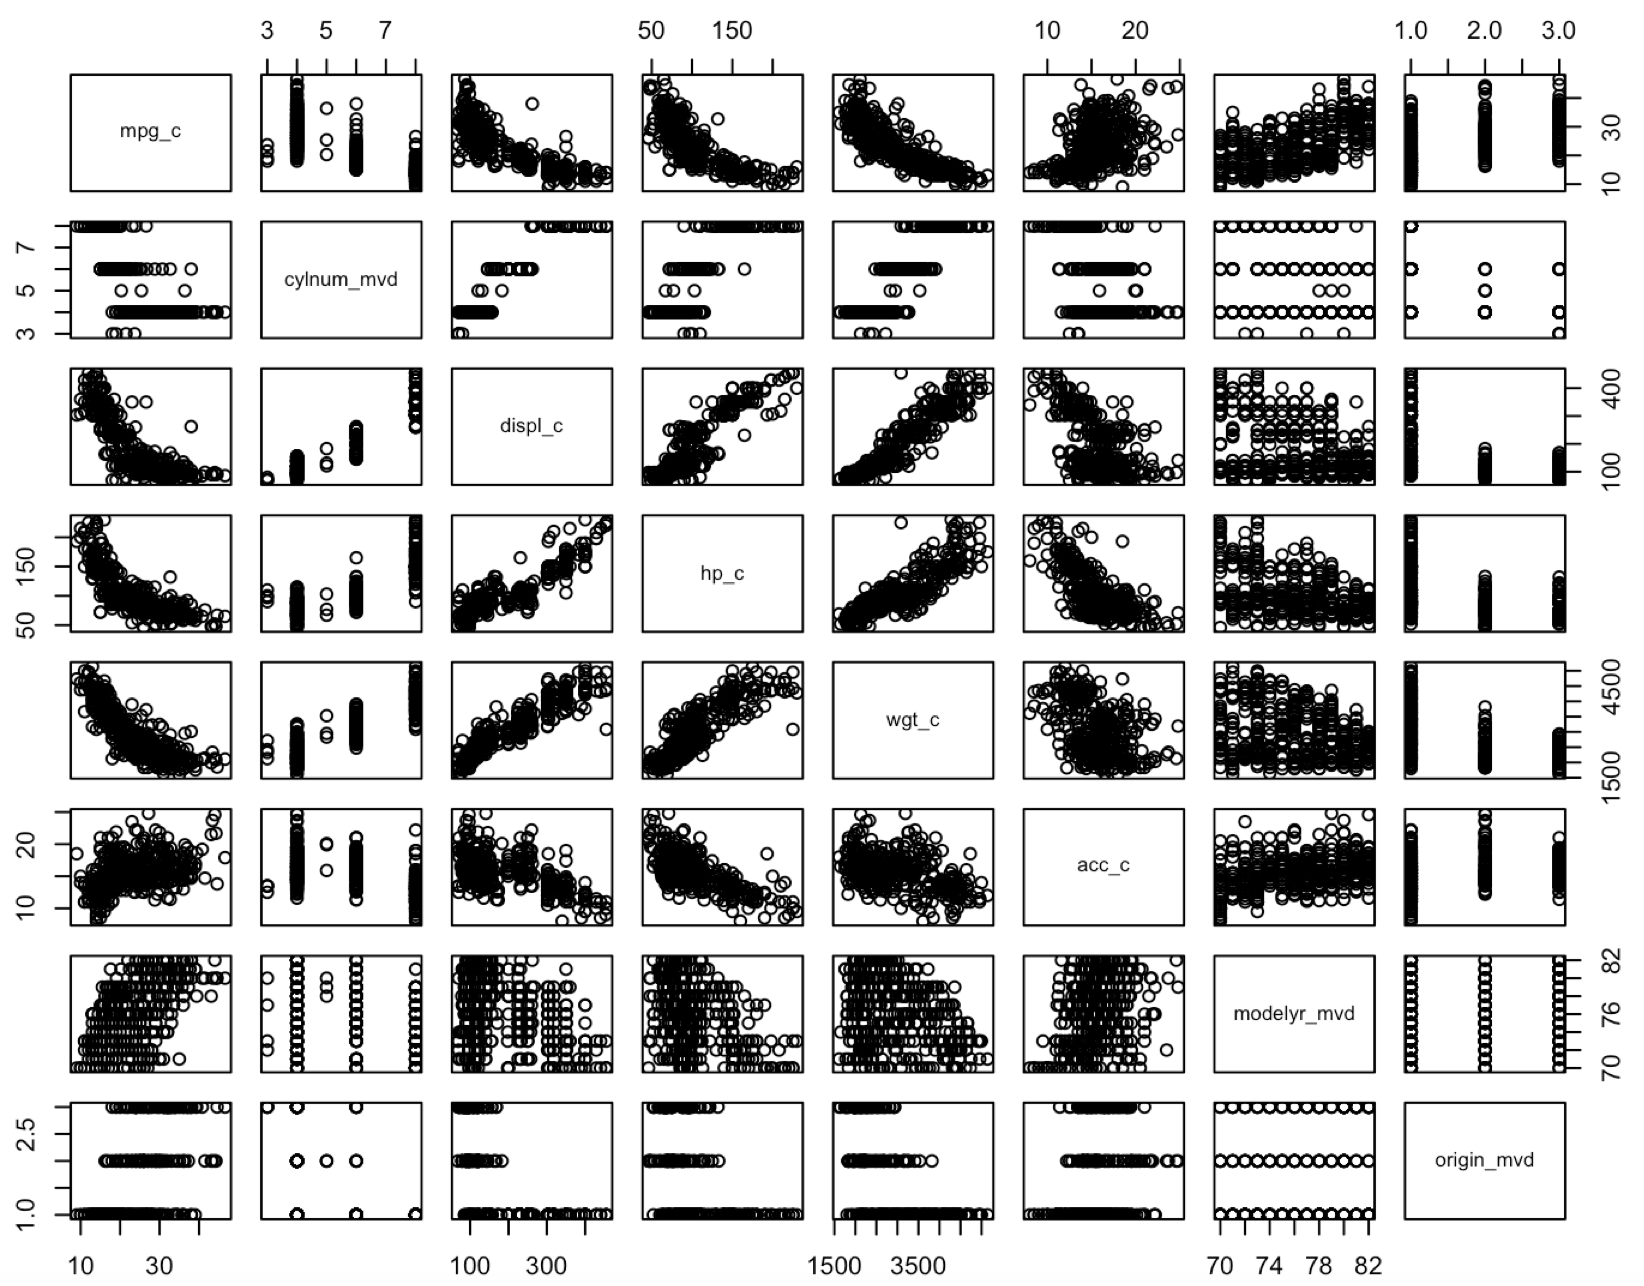
\includegraphics[width=1\linewidth]{1p_ScPlMtr}
	\caption[Scatterplot Matrix of the Original Full Model]
	{A scatterplot matrix between all the variables in the automobile data set}
\end{figure}

\clearpage
\newpage 

\begin{figure}
	\centering
	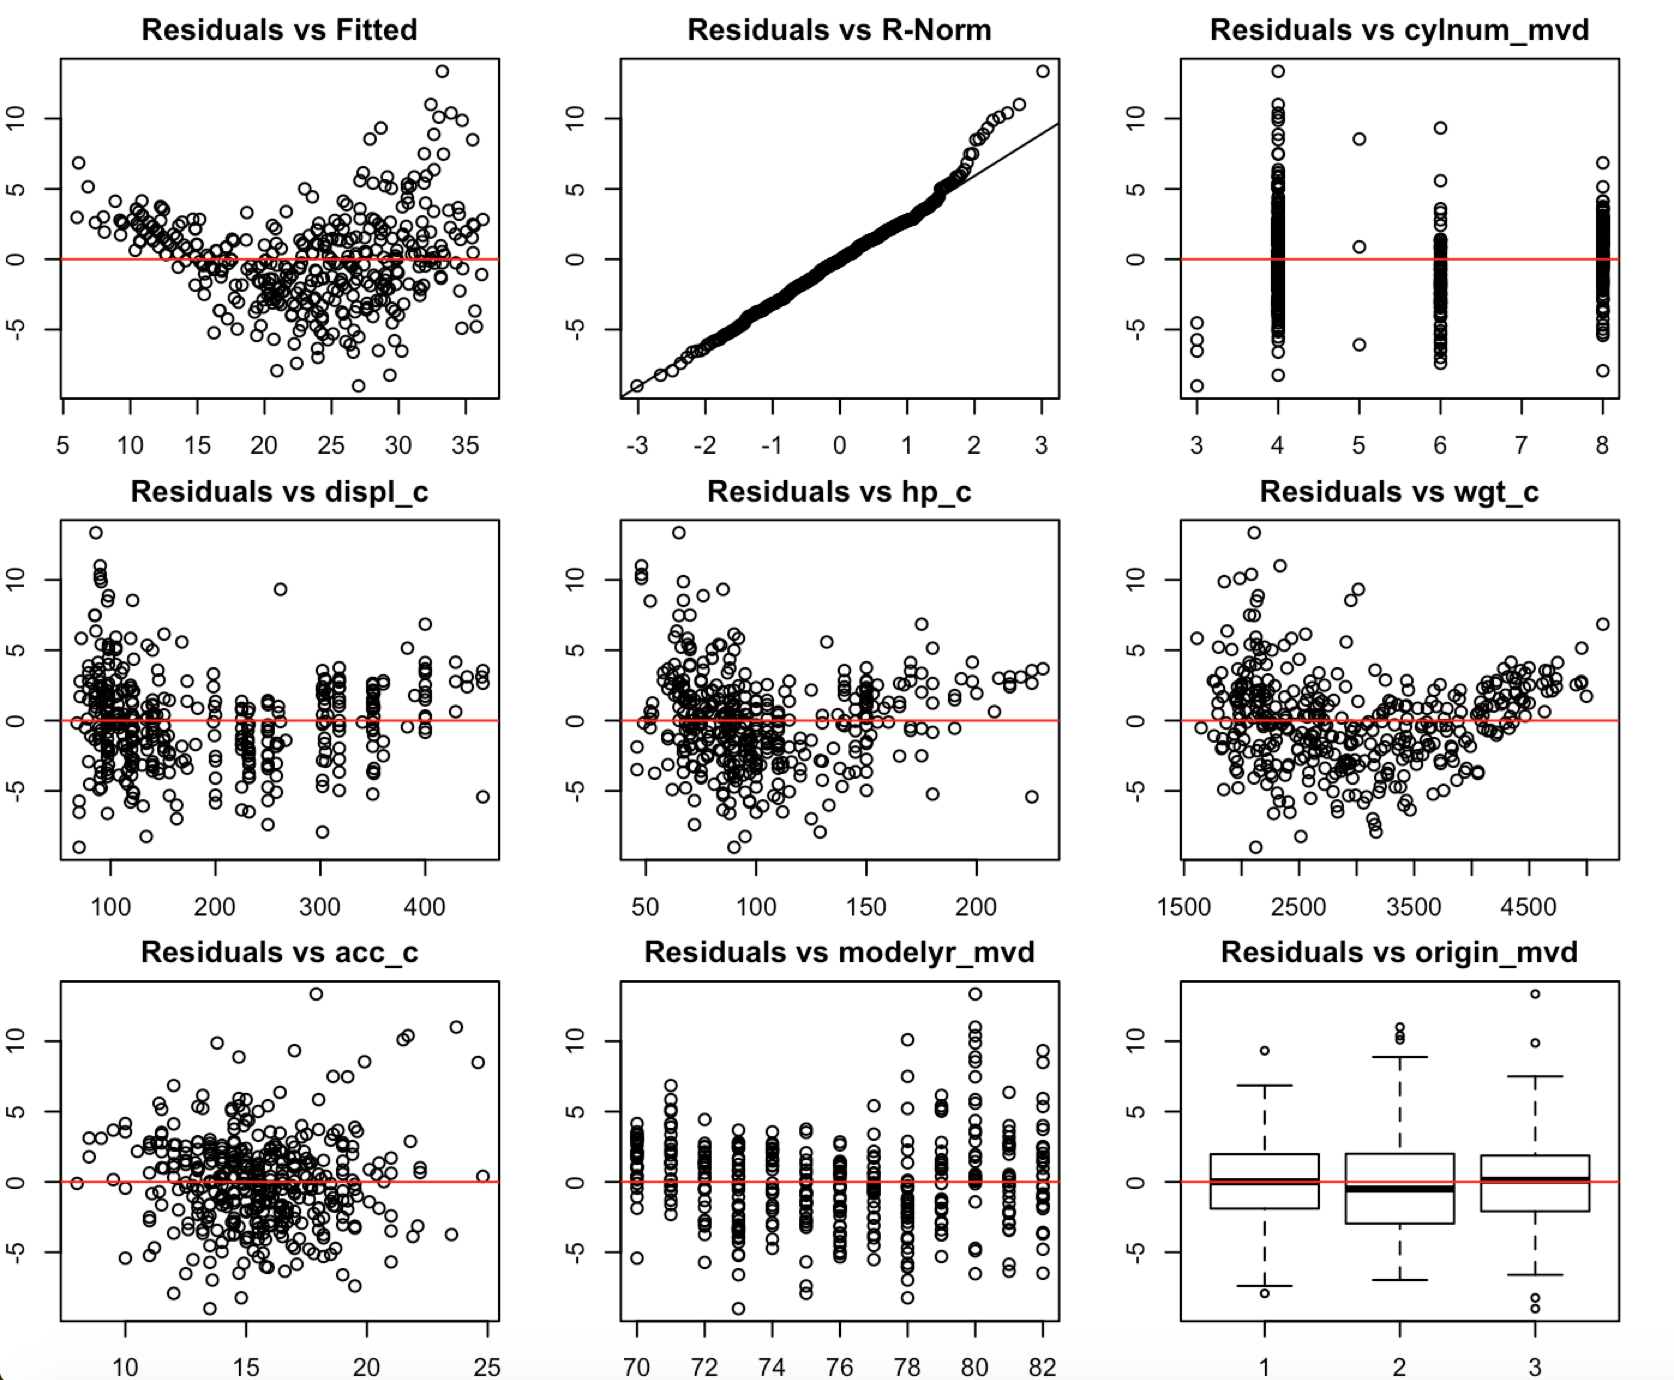
\includegraphics[width=1\linewidth]{2-10p_resall}
	\caption[Residual Plots of the Original Full Model]
	{A Residual vs Fitted, a Residual vs R-Norm, and Residual vs Regressors plots of the Original Full Model}
\end{figure}

\clearpage
\newpage 

\begin{table}[ht]
\centering
\begin{tabular}{rlrrl}
  \hline
 & Regressor & F\_Statistic & P\_Value & Significance \\ 
  \hline
1 & Displacement & 9.89 & 0.00 & ** \\ 
  2 & Weight & 104.63 & 0.00 & *** \\ 
  3 & HP & 1.61 & 0.21 & none \\ 
  4 & Cylinder Num & 2.53 & 0.11 & none \\ 
   \hline
\end{tabular}
\caption{A partial F test on each of the regressors with high VIF scores}
\label{tab:partialfhighvif}
\end{table}

\begin{figure}
	\centering
	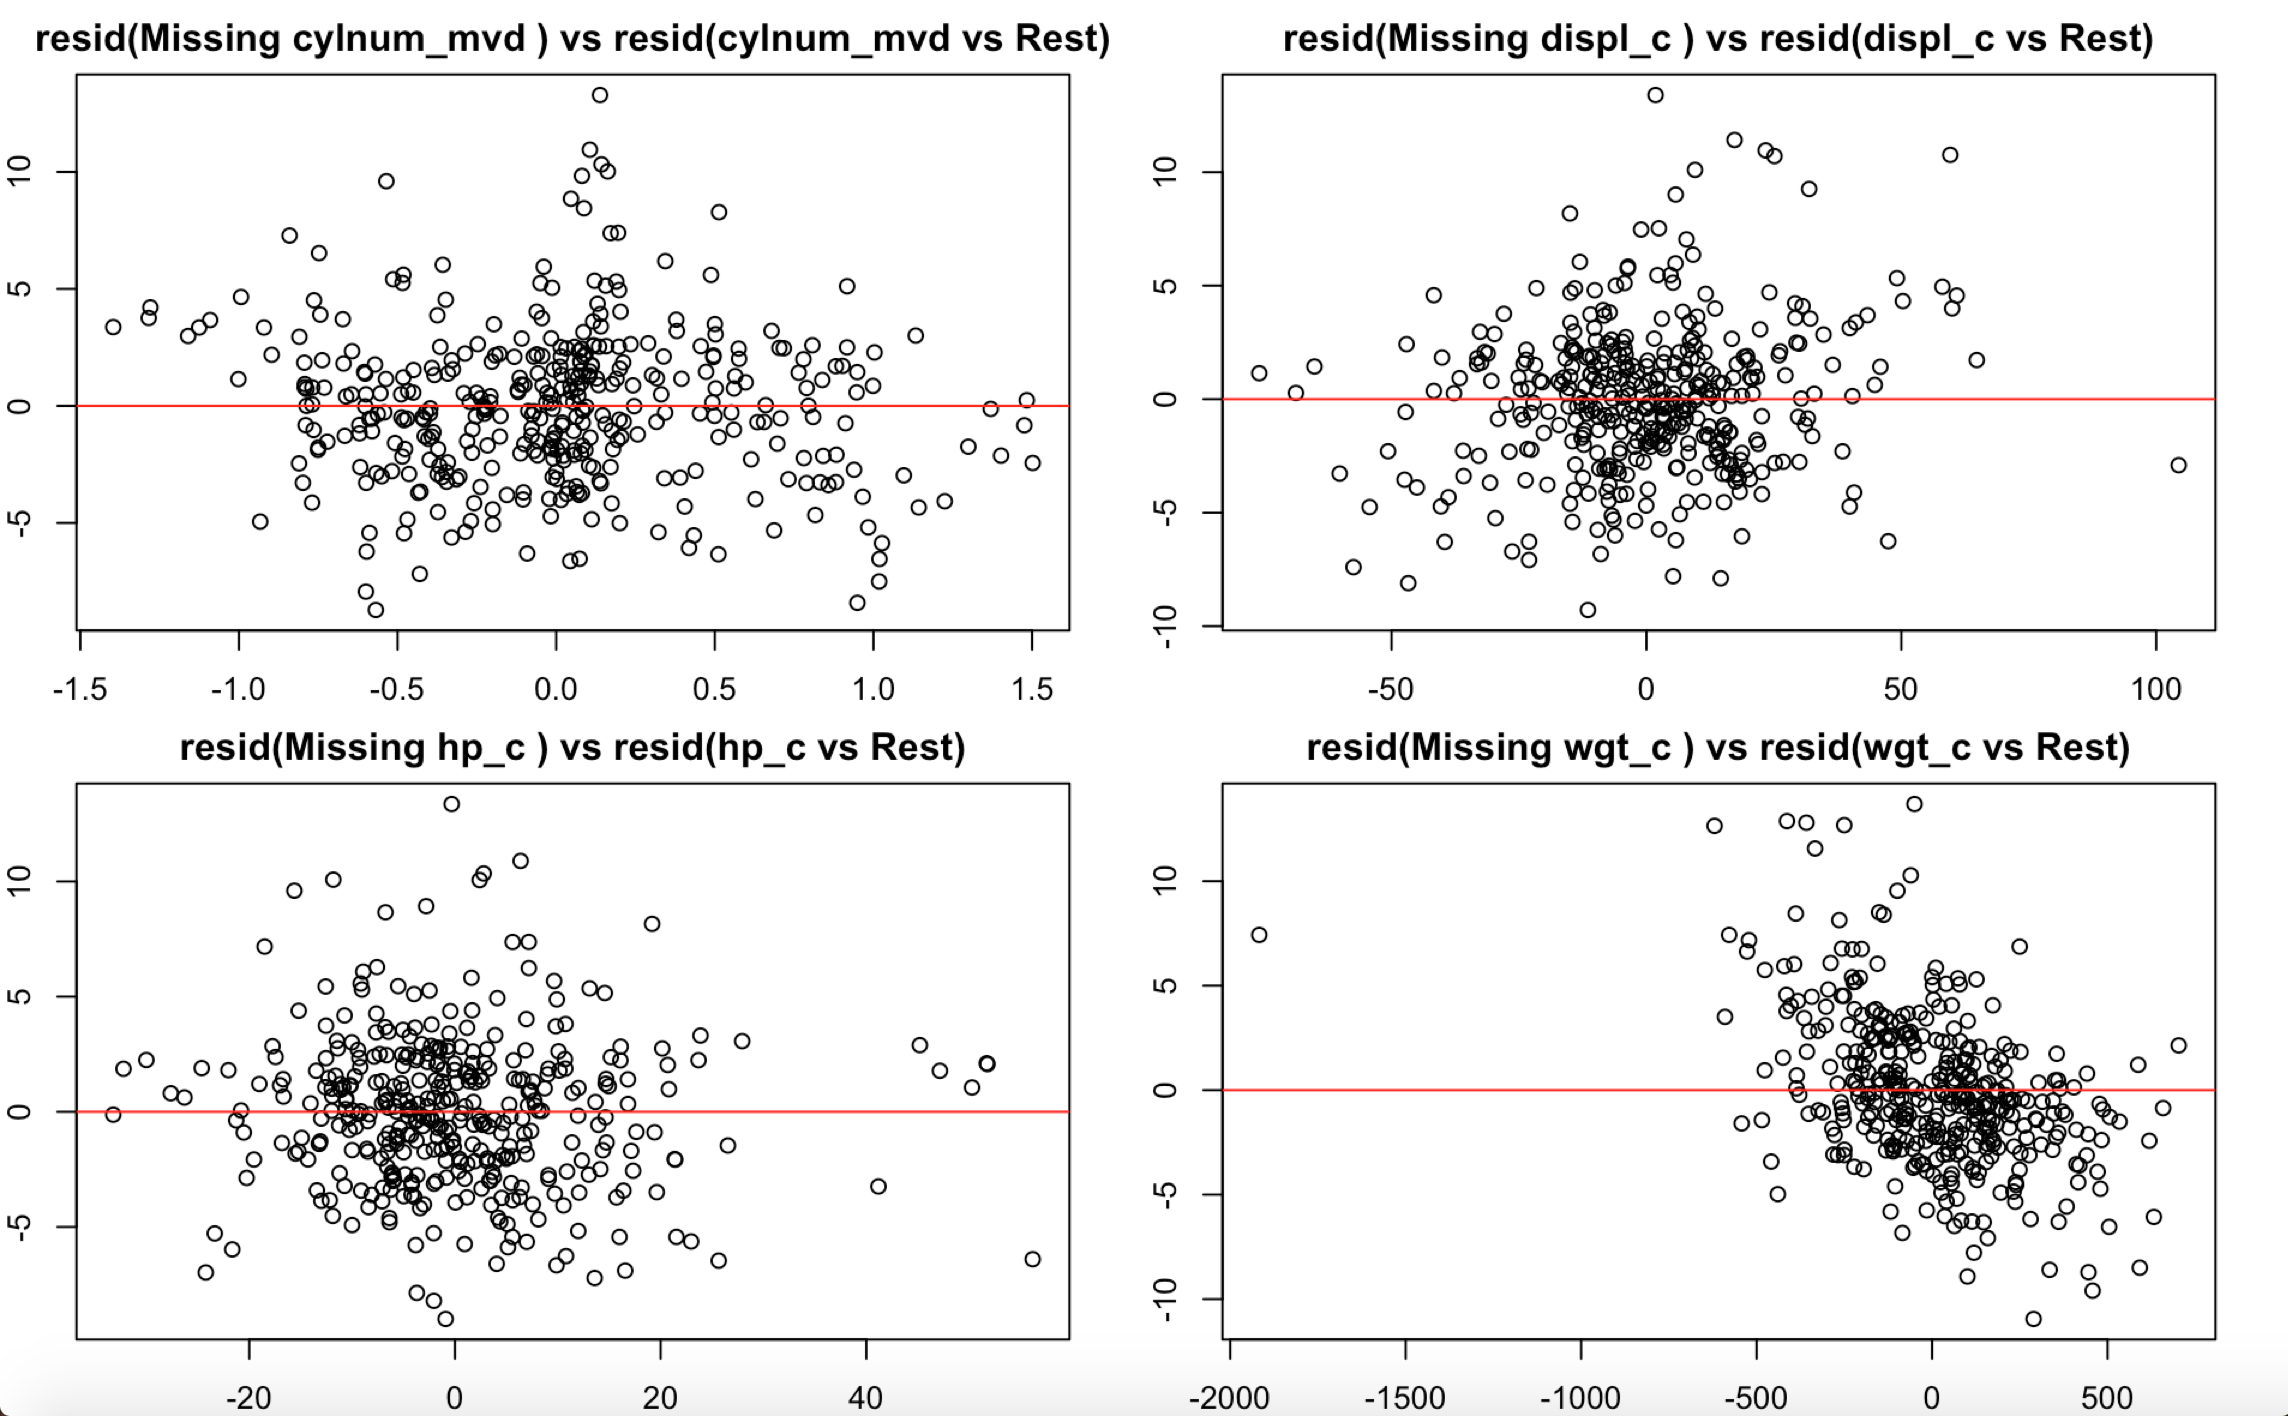
\includegraphics[width=1\linewidth]{11-14p_PrRgall4}
	\caption[Partial regression plots on high VIF regressors]
	{Partial regression plots on each of the regressors with high VIF scores}
\end{figure}

\clearpage
\newpage

Original Model

A multiple linear regression was fitted on miles per gallon ~ number of cylinders (as a factor), displacement, horsepower, weight, acceleration, model year, and origen (as a factor); and the five requirements to realize a regression analysis were checked.

Normality: 

Notice that the Residual vs. Normal plot behaves mostly normal except at the tails. Where the tails seem lighter than the textbook ideal. Yet, this will not bring major issues to the analysis. Therefore, normality can be concluded for this purpose.

Independence, Linearity and Constant Variance:

The Residual vs. Fitted Values plot for this regression,  makes a shoe horse shape plot and, most of the data points are below the abline. It indicates lack of constant variance, non-zero mean error, and a non-linear distribution. This will bring major problems to the predictions, and analysis.  The issue can be addressed in a simple manner; and will be discussed in the next section. Also, notice how all of the residuals are bounded, this is an indication of uncorrelated errors.

Figure 2 and Table 3 gives an insight for correlation among variables. Since a lot of the plots show a linear relationship (with a nonzero slope), multicollinearity is suspected. Further evidence that there exists a dependence among variables are the VIF values of cylinder number, displacement, horsepower and weight; hence it will be needed to include some interaction variables. 


\clearpage 
\newpage

\subsection{Transformed Full Model Analysis}

\textbf{Transformed Full Model:}

\textbf{log(mpg) (c) \tl wgt (c) + modelyr (mvd) + origin (mvd) + hp (c) + displ (c) + cylnum (mvd) + acc (c)}

\begin{figure}[h]
	\centering
	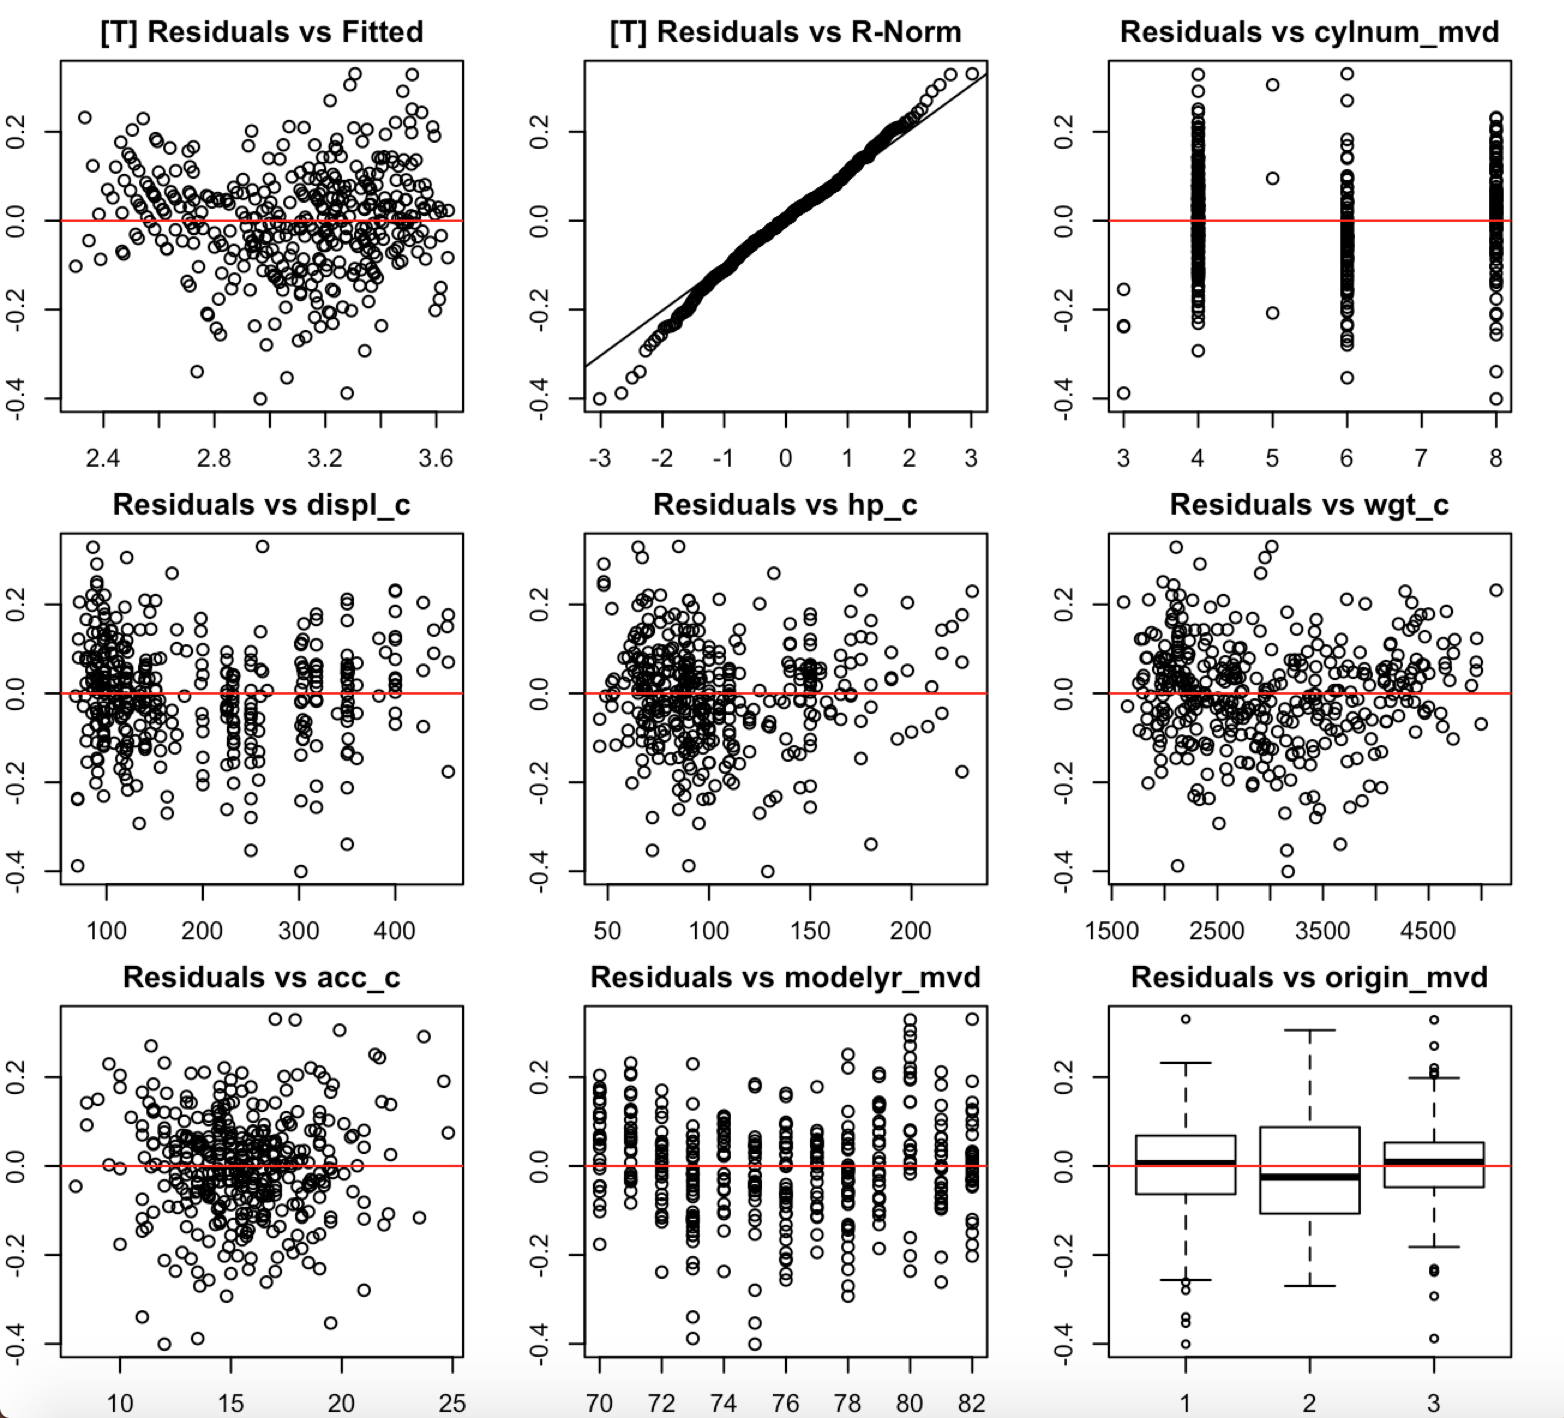
\includegraphics[width=0.95\linewidth]{15-23t_resall}
	\caption[Residual Plots of the Transformed Full Model]
	{A Residual vs Fitted, a Residual vs R-Norm, and Residual vs Regressors plots of the Transformed Full Model}
\end{figure}

\clearpage
\newpage

\begin{table}[ht]
\centering
\begin{tabular}{rlrrl}
  \hline
 & Regressor & F\_Statistic & P\_Value & Significance \\ 
  \hline
1 & Displacement & 8.39 & 0.00 & ** \\ 
  2 & Weight & 126.68 & 0.00 & *** \\ 
  3 & HP & 9.10 & 0.00 & ** \\ 
  4 & Cylinder Num & 6.35 & 0.01 & * \\ 
   \hline
\end{tabular}
\caption{A partial F test on each of the regressors with high VIF scores on the Transformed Full Model}
\label{tab:partialfhighvif}
\end{table}

\begin{figure}
	\centering
	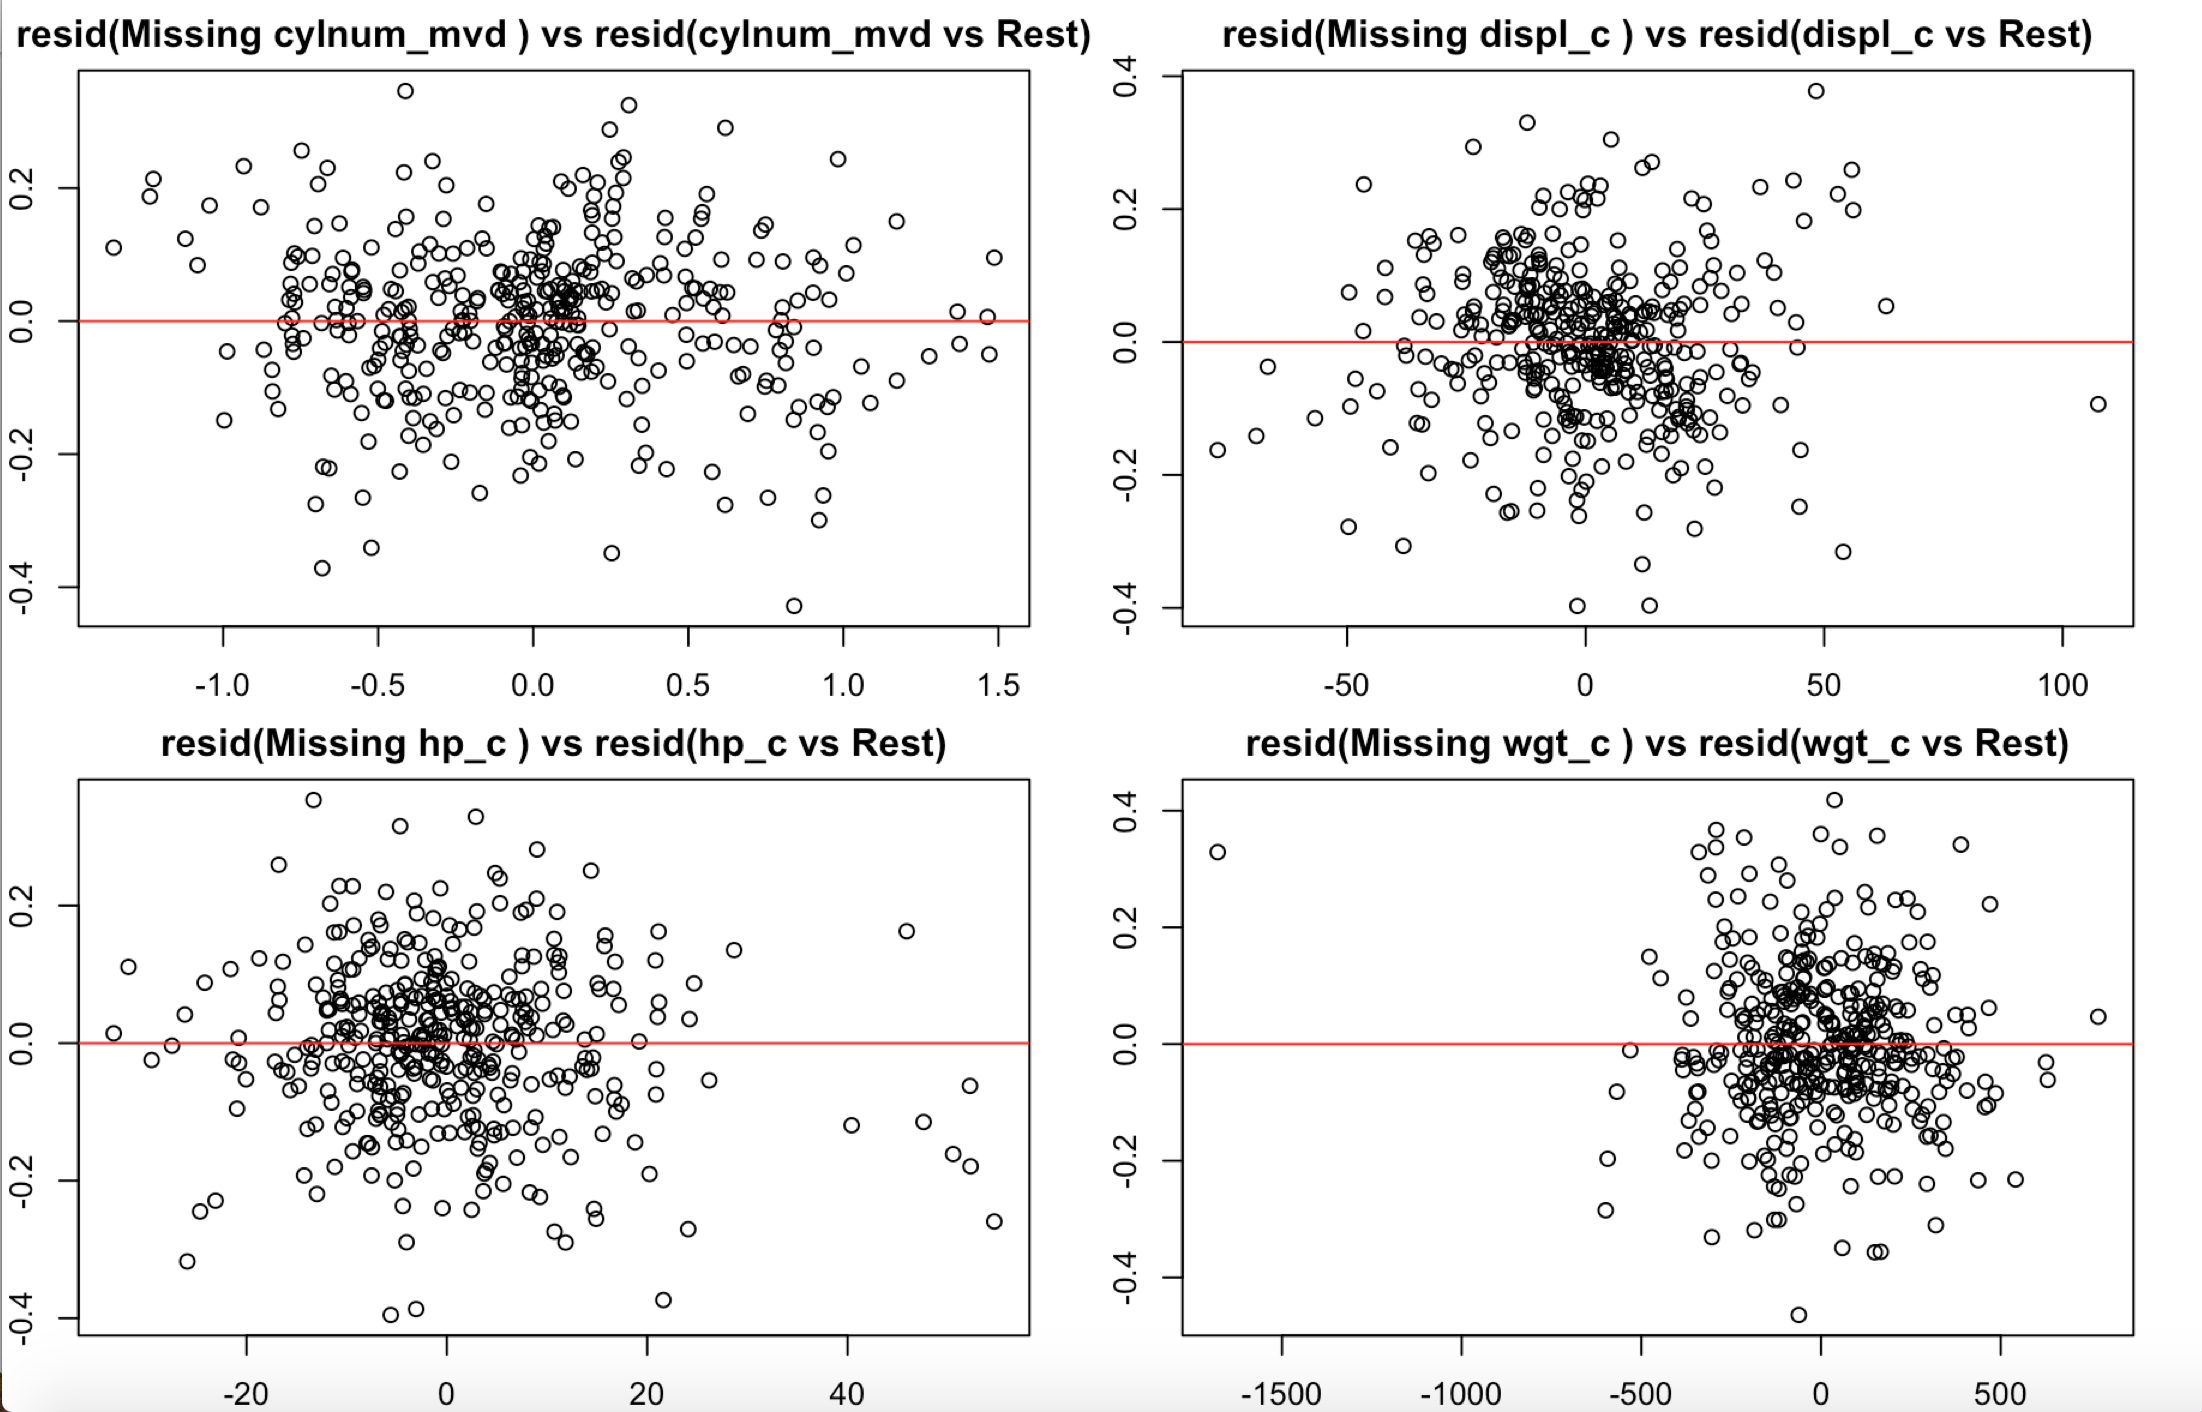
\includegraphics[width=1\linewidth]{24-27t_PrRgall4}
	\caption[Partial regression plots on high VIF regressors on the Transformed Full Model]
	{Partial regression plots on each of the regressors with high VIF scores on the Transformed Full Model}
\end{figure}

\clearpage
\newpage

Several issues, not very major, have been found in the original model. In order to address them a transformation has to be applied into the fit: Since the Residuals vs. Fitted plot showed a horseshoe pattern, based on previous encounters, a log transformation in the predictor was selected:

“Insert transformed regression here”

 Which fixed most of the problems, with regard of the assumptions:
 
Figure 4, Residuals vs. Fitted shows that the new model  is linear, has mean zero error, and independent .


Notice, in Figure 4 Residuals vs. R-Norm, that a new problem has arised in the tails have become lighter, compared to the original.  This could be caused by interaction among variables and/or influential points. It is worth to remark that in this model, so far cylinder number, horsepower, and weight do not contribute much towards the model: based on the partial residual plots (Figure 5), there is no apparent pattern on said variables. But, the partial F-Test indicates otherwise, which is a stronger sign of interaction.

The remainder of the plots, show a constant band of residuals, which is a sign of constant variance. 
	 Thus, based on all of the previews evidence there must be variables interacting with each other, and should be included in the model. 

\clearpage
\newpage

\subsection{Interaction Terms Analysis}

\begin{table}[ht]
\centering
\begin{tabular}{rlrrr}
  \hline
 & Model & R\_Sq & AR\_Sq & MS\_res \\ 
  \hline
1 & Interaction & 0.88 & 0.87 & 7.90 \\ 
  2 & Transformed + Interaction & 0.90 & 0.90 & 0.01 \\ 
   \hline
\end{tabular}
\caption{A chart comparing the Untransformed Full Model with all combinations of interaction terms for the high VIF regressors against the same model with a log transformation on the response variable (mpg)}
\label{tab:myfirsttable}
\end{table}

\newpage

\subsection{Model Selection Analysis}

\begin{table}[ht]
\centering
\begin{tabular}{rlrrrr}
  \hline
 & Selection\_Method & Num\_Regressors & R\_Sq & Adj\_R\_Sq & MS\_res \\ 
  \hline
1 & Forward & 6.00 & 0.89 & 0.89 & 0.01 \\ 
  2 & Backward & 16.00 & 0.90 & 0.90 & 0.01 \\ 
  3 & Stepwise & 6.00 & 0.89 & 0.89 & 0.01 \\ 
   \hline
\end{tabular}
\caption{Statistics about the models outputted from Forward, Backward, and Stepwise Selection algorithms in R (note that the model selected by Forward and Stepwise selection is identical, so just the Forward model will be considered in further sections)}
\label{tab:myfirsttable}
\end{table}

\begin{table}[ht]
\centering
\begin{tabular}{rrrr}
  \hline
 & GVIF & Df & GVIF\verb|^|(1/(2*Df)) \\ 
  \hline
wgt\_c & 13.83 & 1.00 & 3.72 \\ 
  modelyr\_mvd & 1.27 & 1.00 & 1.13 \\ 
  origin\_mvd & 1.74 & 2.00 & 1.15 \\ 
  hp\_c & 37.47 & 1.00 & 6.12 \\ 
  acc\_c & 2.61 & 1.00 & 1.62 \\ 
  wgt\_c:hp\_c & 58.06 & 1.00 & 7.62 \\ 
   \hline
\end{tabular}
\caption{VIF of each regressor in the Forward Model}
\label{tab:forwardmodelvif}
\end{table}

\begin{table}[ht]
\centering
\begin{tabular}{rrrr}
  \hline
 & GVIF & Df & GVIF\verb|^|(1/(2*Df)) \\ 
  \hline
wgt\_c & 3110.02 & 1.00 & 55.77 \\ 
  modelyr\_mvd & 1.44 & 1.00 & 1.20 \\ 
  origin\_mvd & 3.01 & 2.00 & 1.32 \\ 
  hp\_c & 2806.06 & 1.00 & 52.97 \\ 
  displ\_c & 10568.29 & 1.00 & 102.80 \\ 
  cylnum\_mvd & 975.92 & 1.00 & 31.24 \\ 
  acc\_c & 3.64 & 1.00 & 1.91 \\ 
  wgt\_c:hp\_c & 27058.36 & 1.00 & 164.49 \\ 
  hp\_c:displ\_c & 39680.75 & 1.00 & 199.20 \\ 
  wgt\_c:displ\_c & 11724.72 & 1.00 & 108.28 \\ 
  wgt\_c:cylnum\_mvd & 9069.37 & 1.00 & 95.23 \\ 
  hp\_c:cylnum\_mvd & 9125.25 & 1.00 & 95.53 \\ 
  displ\_c:cylnum\_mvd & 19861.83 & 1.00 & 140.93 \\ 
  wgt\_c:hp\_c:cylnum\_mvd & 41867.56 & 1.00 & 204.62 \\ 
  wgt\_c:displ\_c:cylnum\_mvd & 15077.88 & 1.00 & 122.79 \\ 
  hp\_c:displ\_c:cylnum\_mvd & 44842.29 & 1.00 & 211.76 \\ 
   \hline
\end{tabular}
\caption{VIF of each regressor in the Backward Model}
\label{tab:backwardmodelvif}
\end{table}

\clearpage
\newpage 

\begin{figure}
	\centering
	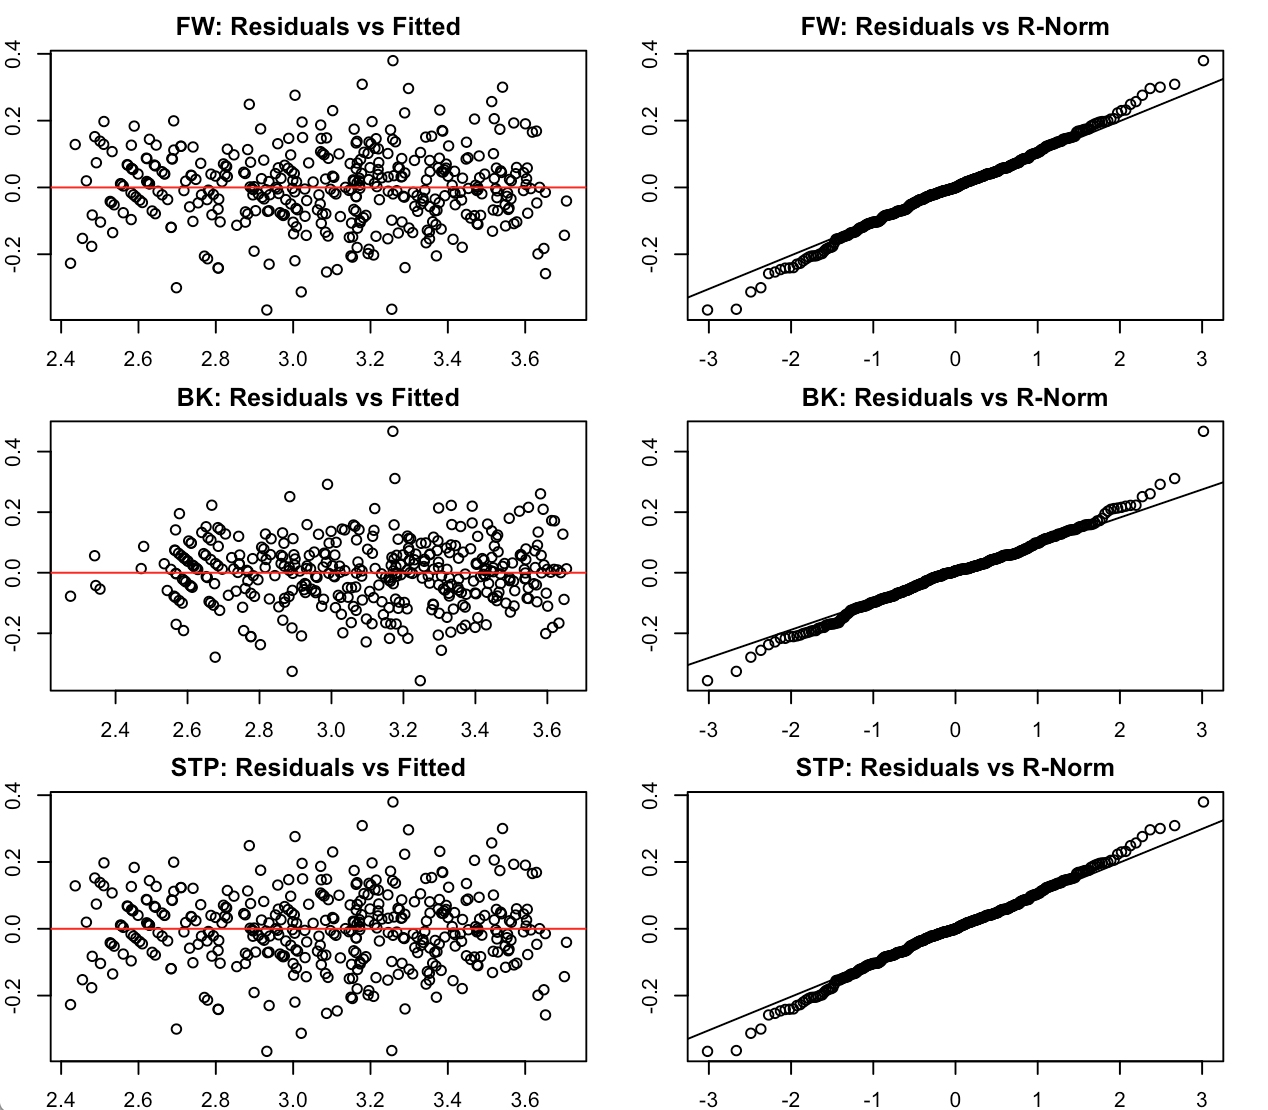
\includegraphics[width=1\linewidth]{28ti_resfittednorm}
	\caption[Residuals vs Fitted and vs Random Normal plots for Forward, Backward, and Stepwise Models]
	{Residuals vs Fitted and vs Random Normal plots for Forward, Backward, and Stepwise Models}
\end{figure}

\clearpage
\newpage 

\subsection{Influential Points Analysis}

\begin{table}[ht]
\centering
\begin{tabular}{rlrlr}
  \hline
 & Model & Num\_Infl\_Pnts & Percent\_Infl\_Pnts & Common\_Infl\_Pnts \\ 
  \hline
1 & Forward & 20.00 & 5.12\% & 14.00 \\ 
  2 & Backward & 36.00 & 9.21\% & 14.00 \\ 
   \hline
\end{tabular}
\caption{Influential point comparison of Forward Model vs Backward Model}
\label{tab:myfirsttable}
\end{table}

\begin{table}[ht]
\centering
\begin{tabular}{rlrrr}
  \hline
 & Model & R\_Sq & AR\_Sq & MS\_res \\ 
  \hline
1 & Forward w/o Infl & 0.91 & 0.91 & 0.01 \\ 
  2 & Backward w/o Infl & 0.90 & 0.90 & 0.01 \\ 
   \hline
\end{tabular}
\caption{Forward Model with no influential points vs Backward Model with no influential points}
\label{tab:forwardvsbackwardnoinfluential}
\end{table}

\clearpage
\newpage

\subsection{Final Model Choice}

\textbf{FINAL MODEL: log(mpg) (c) \tl modelyr (mvd) + origin (mvd) + hp (c) + acc (c) + wgt (c) * hp (c)}

\begin{table}[ht]
\centering
\begin{tabular}{rrrrrr}
  \hline
 & Estimate & Std. Error & t value & Pr($>$$|$t$|$) & Significance\\ 
  \hline
(Intercept) & 2.1373 & 0.1735 & 12.32 & 0.00001 & *** \\ 
  wgt\_c & -0.0004 & 0.0000 & -14.76 & 0.00001 & *** \\ 
  modelyr\_mvd & 0.0309 & 0.0018 & 17.59 & 0.00001 & *** \\ 
  origin\_mvd2 & 0.0558 & 0.0177 & 3.14 & 0.00180 & ** \\ 
  origin\_mvd3 & 0.0455 & 0.0180 & 2.52 & 0.01210 & * \\ 
  hp\_c & -0.0064 & 0.0009 & -7.06 & 0.00001 & *** \\ 
  acc\_c & -0.0053 & 0.0034 & -1.59 & 0.11180 & \\ 
  wgt\_c:hp\_c & 0.0000013 & 0.0000002 & 6.71 & 0.00001 & *** \\ 
   \hline
\end{tabular}
\caption{R Summary of the final model}
\label{tab:summaryfinalmodel}
\end{table}

\begin{table}[ht]
\centering
\begin{tabular}{lrrrrrr}
  \hline
 & Df & Sum Sq & Mean Sq & F value & Pr($>$F) & Significance \\ 
  \hline
wgt\_c & 1 & 34.62 & 34.62 & 2714.64 & 0.0000 & *** \\ 
  modelyr\_mvd & 1 & 4.72 & 4.72 & 369.94 & 0.0000 & *** \\ 
  origin\_mvd & 2 & 0.25 & 0.12 & 9.78 & 0.0001 & *** \\ 
  hp\_c & 1 & 0.11 & 0.11 & 8.87 & 0.0031 & ** \\ 
  acc\_c & 1 & 0.001 & 0.00 & 0.26 & 0.6078 & \\ 
  wgt\_c:hp\_c & 1 & 0.57 & 0.57 & 45.04 & 0.0000 & *** \\ 
  Residuals & 383 & 4.88 & 0.01 &  &  & \\ 
   \hline
\end{tabular}
\caption{R ANOVA of the final model}
\label{tab:anovafinalmodel}
\end{table}

\section{Conclusion}

\section{References}

\end{document}